
include(`macros.m4')

\pagebreak
\pdfbookmark[0]{network programming}{site}

\begin{slide}
\sltitle{Contents}
\slidecontents{7}
\end{slide}

%%%%%%%%%%%%%%%%%%%%%%%%%%%%%%%%%%%%%%%%%%%%%%%%%%%%%%%%%%%%%%%%%%%%%%%%%

\label{NETWORKING}

\begin{slide}
\sltitle{Network communication}
\begin{description}
\item[UUCP (UNIX-to-UNIX Copy Program)] -- first application for communication
between UNIX systems connected directly or via modems, in Version~7 UNIX (1978)
\item[sockets] -- introduced in 4.1 BSD (1982); socket is one end of a
bidirectional communication channel created between two processes either on the
same computer or across a network.
\item[TLI (Transport Layer Interface)] -- SVR3 (1987); API providing network
communication within the \nth{4} layer of ISO OSI.  Counterpart to the BSD
sockets API.
\item[RPC (Remote Procedure Call)] -- SunOS (1984); provides access to services
running on a remote machine, data transferred in XDR format (External Data
Representation)
\end{description}
\end{slide}

\begin{itemize}
\item There are two main conceptual models for network communication.  ISO
(International Standards Organization) OSI (Open Systems Interconnect), and the
Internet protocol suite (also called TCP/IP).   Each one defines several layers.
If we oversimplify, ISO OSI is very formal, quite complex, has 7 layers, and its
specification is not freely available, while TCP/IP is simpler, not that formal,
with 4 layers, and the specification is freely available via RFCs.  While the
layers of the two models cannot be precisely mapped onto each other, the
corresponding layers are roughly as follows:

\vspace{1.5mm}

\renewcommand{\arraystretch}{1.2}
\begin{tabular}{|l|l|}\hline
ISO OSI & TCP/IP\\
\hline
\hline
application & application\\
presentation & \\
session & \\
\hline
transport & transport\\
\hline
network & internet\\
\hline
link & link\\
physical & \\
\hline
\end{tabular}
\renewcommand{\arraystretch}{1}

\vspace{1.5mm}

We will be working exclusively with the TCP/IP model.

\item UUCP is a historical thing, fully implemented in userland without any
kernel support.  See the \texttt{uucp} man page or Wikipedia for more
information.
\item RPC is implemented as a library linked to applications, uses sockets
and works on top of TCP and UDP.  RPC was developed as a communication protocol
for the \emph{Network Filesystem} (NFS).  There are several mutually
incompatible RPC implementations.
\item TLI is designed from an OSI model-oriented viewpoint, and it corresponds
to the \nth{4} layer -- transport.  TLI API looks similar to sockets.
\item Sockets for communication within the same host are in the
\texttt{AF\_UNIX} domain and their names correspond to special files that
represent the sockets in the filesystem.  \texttt{ls -F} uses the equal sign
``='' to mark a Unix domain socket.
\item Sockets in \texttt{AF\_UNIX} are different from local TCP/IP communication
over the loopback interface \texttt{localhost} (\texttt{127.0.0.1}).  See page
\pageref{SOCKET} for more information on \texttt{AF\_UNIX}.
\end{itemize}

%%%%%

\begin{slide}
\sltitle{TCP/IP basics}
\begin{itemize}
\item protocols
    \begin{itemize}
    \item \emsl{IP (Internet Protocol)} -- principal communications protocol,
    not accessible for a non-privileged user
    \item \emsl{TCP (Transmission Control Protocol)} -- reliable, ordered, and
    error-checked delivery of a stream of bytes
    \item \emsl{UDP (User Datagram Protocol)} -- datagram, connection-less,
    unreliable
    \end{itemize}
\item \emsl{IP address} -- 4 bytes (IPv4) / 16 bytes (IPv6), defines a network
interface, not a computer
\item \emsl{port} -- 2 bytes, application end-points on a host
\item \emsl{DNS (Domain Name System)} --  translates domain names to the
numerical IP addresses 
\end{itemize}
\end{slide}

\begin{itemize}
\item Unix mostly uses protocols from the TCP/IP family.  We will cover TCP and
UDP.  In both protocols, one end of a communication channel is identified by an
IP address and a port.  Those two pieces correspond to a socket.  A TCP
connection is uniquely identified by a pair of sockets.
\item Ports below 1024 are reserved and additional privileges are needed to use
them.  For example, \emph{root} can access those.  See \texttt{/etc/services}
for the textual database of port numbers and corresponding service names.
\item To learn about networking and the Internet in general, we very much
recommend networking lectures by
ifdef([[[NOSPELLCHECK]]], [[[Ji\v{r}\'{i} Peterka]]]).  You can either
attend them at MFF~UK or you can find those online.
\item \emph{IP} -- protocol of the internet layer within the TCP/IP network
stack, provides data transfer between two interfaces identified by an IP
address.  It is unreliable.  Provides routing and fragmentation.  Defined in
RFC~791.  The Internet Control Message Protocol (ICMP), defined in RFC~792, is
an inherent part of the IP protocol.
\item \emph{UDP} -- a simple extension of the IP protocol, only adds protocol
numbers.  Still unreliable and datagram oriented.  Defined in RFC~768.
\item \emph{TCP} -- establishes connections between two points (sockets).
Provides a continuous stream of data, congestion control and reliable
delivery.  To create a connection, a so called \emph{handshake} must be
performed.  The protocol is defined in RFC~793 and other follow-up RFCs.
\item \emph{DNS} -- hierarchically organized database, its structure does not
have to follow the IP address structure.
\end{itemize}

%%%%%

\begin{slide}
\sltitle{Connection-oriented (TCP), sequential service}
\begin{picture}(0,0)%
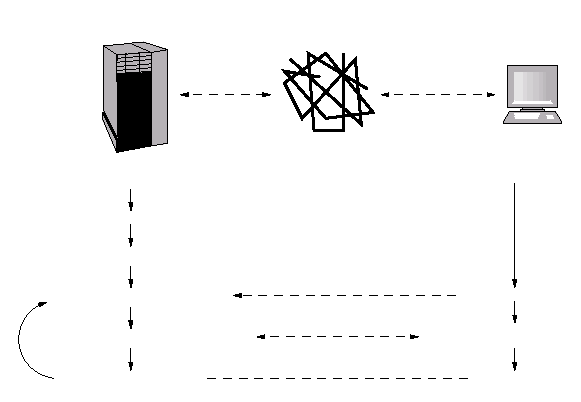
\includegraphics{img/tex/tcp_seq}%
\end{picture}%
\setlength{\unitlength}{4144sp}%
%
\begingroup\makeatletter\ifx\SetFigFont\undefined%
\gdef\SetFigFont#1#2#3#4#5{%
  \reset@font\fontsize{#1}{#2pt}%
  \fontfamily{#3}\fontseries{#4}\fontshape{#5}%
  \selectfont}%
\fi\endgroup%
\begin{picture}(4157,2790)(-8,-2041)
\put(406,-511){\makebox(0,0)[lb]{\smash{\SetFigFont{10}{12.0}{\ttdefault}{\mddefault}{\updefault}{\color[rgb]{0,0,0}fd = socket()}%
}}}
\put(541,-1123){\makebox(0,0)[lb]{\smash{\SetFigFont{10}{12.0}{\ttdefault}{\mddefault}{\updefault}{\color[rgb]{0,0,0}listen(fd)}%
}}}
\put(631,-817){\makebox(0,0)[lb]{\smash{\SetFigFont{10}{12.0}{\ttdefault}{\mddefault}{\updefault}{\color[rgb]{0,0,0}bind(fd)}%
}}}
\put(271,-1429){\makebox(0,0)[lb]{\smash{\SetFigFont{10}{12.0}{\ttdefault}{\mddefault}{\updefault}{\color[rgb]{0,0,0}fd2 = accept(fd)}%
}}}
\put( 46,-1735){\makebox(0,0)[lb]{\smash{\SetFigFont{10}{12.0}{\ttdefault}{\mddefault}{\updefault}{\color[rgb]{0,0,0}read(fd2); write(fd2)}%
}}}
\put(541,-2041){\makebox(0,0)[lb]{\smash{\SetFigFont{10}{12.0}{\ttdefault}{\mddefault}{\updefault}{\color[rgb]{0,0,0}close(fd2)}%
}}}
\put(3331,-511){\makebox(0,0)[lb]{\smash{\SetFigFont{10}{12.0}{\ttdefault}{\mddefault}{\updefault}{\color[rgb]{0,0,0}fd = socket()}%
}}}
\put(3511,-2041){\makebox(0,0)[lb]{\smash{\SetFigFont{10}{12.0}{\ttdefault}{\mddefault}{\updefault}{\color[rgb]{0,0,0}close(fd)}%
}}}
\put(3106,-1726){\makebox(0,0)[lb]{\smash{\SetFigFont{10}{12.0}{\ttdefault}{\mddefault}{\updefault}{\color[rgb]{0,0,0}write(fd);read(fd)}%
}}}
\put(3421,-1411){\makebox(0,0)[lb]{\smash{\SetFigFont{10}{12.0}{\ttdefault}{\mddefault}{\updefault}{\color[rgb]{0,0,0}connect(fd)}%
}}}
\put(721,659){\makebox(0,0)[lb]{\smash{\SetFigFont{10}{12.0}{\sfdefault}{\mddefault}{\updefault}{\color[rgb]{0,0,0}server}%
}}}
\put(3736,569){\makebox(0,0)[lb]{\smash{\SetFigFont{10}{12.0}{\sfdefault}{\mddefault}{\updefault}{\color[rgb]{0,0,0}klient}%
}}}
\put(2206,569){\makebox(0,0)[lb]{\smash{\SetFigFont{10}{12.0}{\sfdefault}{\mddefault}{\updefault}{\color[rgb]{0,0,0}s��}%
}}}
\end{picture}

\end{slide}

\begin{itemize}
\item Note that common \funnm{read}() a \funnm{write}() calls are used.  To
keep the picture readable, all arguments aside from a descriptor \emph{fd} were
intentionally omitted.
\item The server creates one connection and does not accept a new one until the
previous connection finished.  That is why it is called a sequential service.
\item System calls used:
\begin{itemize}
\item \funnm{socket}() -- creates a socket, returns its descriptor.

\item \funnm{bind}() -- binds an IP address and a port number with the socket.
In other words, it assigns a name to an unnamed socket.  The address must be
either one of IP addresses assigned to one of the host network interfaces (the
host where the socket was created), in which case it will only accept connection
requests over that specific interface via that specific IP address, or it can be
a special value \texttt{INADDR\_ANY} (for so called \emph{wildcard sockets},
denoting the connection will be accepted on any IP address on any interface of
the host.
\item \funnm{listen}() -- tells the kernel to start listening on connection
requests on the socket.
\item \funnm{accept}() -- blocks the process until there is a connection
request, then creates the connection and returns a \emsl{new} descriptor which
is used for communicating with the client.  The original socket descriptor can
be used for another \funnm{accept}() call to serve a new connection request from
another client.
\item \funnm{close}() -- closes the connection.
\item \funnm{connect}() -- the client asks to create a connection.  The IP
address and a port number are passed as arguments (omitted in the picture), the
communication is performed through an already existing socket descriptor
\emph{fd}.  In contrast to \funnm{accept}(), a new file descriptor is not
created.
\end{itemize}
\end{itemize}

%%%%%

\pdfbookmark[1]{socket}{socket}

\begin{slide}
\sltitle{Creating a socket: \texttt{socket()}}
\setlength{\baselineskip}{0.9\baselineskip}
\texttt{int \funnm{socket}(int \emph{domain}, int \emph{type},
int \emph{protocol});}
\begin{itemize}
\item creates a socket, returns its descriptor
\item \emph{domain} -- ,,where the communication will take place'': 
    \begin{itemize}
    \item \texttt{AF\_UNIX} \dots{} local communication within a host, its
    address is a file name. Also \texttt{AF\_LOCAL}.
    \item \texttt{AF\_INET}, \texttt{AF\_INET6} \dots{} internet communication,
    the address is an IP address and port pair
    \end{itemize}
\item \emph{type}:
    \begin{itemize}
    \item \texttt{SOCK\_STREAM} \dots{} connection-oriented reliable service,
    provides bidirectional data stream
    \item \texttt{SOCK\_DGRAM} \dots{} connection-less unreliable service,
    transmits datagram
    \end{itemize}
\item \emph{protocol}: \texttt{0} (default for a given \emph{type})
or a valid protocol number (e.g. \texttt{6}~=~TCP, \texttt{17}~=~UDP)
\end{itemize}
\end{slide}

\label{SOCKET}

\begin{itemize}
\item Function is declared in \texttt{<sys/socket.h>} as well as other network
related functions from the previous slide.
\item Sockets use the same name space as file descriptors, i.e. the same
descriptor table.  If you write a simple program that only calls
\funnm{socket}(), it will return 3 as that will be the first available slot in
the descriptor table.
\item Connection-oriented communication is always bidirectional and is similar
to pipes.  However, note that pipes may not be bidirectional, see page
\pageref{TWO_WAY_PIPES}.
\item Sometimes you can see constants beginning with \verb#PF_# (meaning
\emph{protocol family}, e.g. \texttt{PF\_IN\-ET}, \verb#PF_UNIX#, or
\texttt{PF\_IN\-ET6}) and used in a \funnm{socket}() call. Constants \verb#AF_#
(\emph{address family}) are then used only for naming the sockets.  While it
might make a better sense, the UNIX specification only defines \verb#AF_#
constants.  And if \verb#PF_# constants exist on a system, they are defined via
corresponding \verb#AF_# constants.  We do recommend to use only \verb#AF_#
constants.
\item There are other domains, see the \texttt{socket(2)} manual page.
\item There are also other socket types, for example \texttt{SOCK\_RAW}, for
full protocol access. In order to use \texttt{SOCK\_RAW} you usually need
additional privileges.  That is a reason why a command \texttt{ping}, which
works with ICMP headers of sent packets, might need an SUID privilege:

\begin{verbatim}
$ ls -l /usr/sbin/ping
-r-sr-xr-x   1 root  bin  55680 Nov 14 19:01 /usr/sbin/ping
\end{verbatim}
\end{itemize}

%%%%%

\pdfbookmark[1]{bind}{bind}

\begin{slide}
\sltitle{Naming the socket: \texttt{bind()}}
ifdef([[[NOSPELLCHECK]]], [[[
\funml{int \funnm{bind}(\=int \emph{socket},
const struct sockaddr *\emph{address}, \\\>socklen\_t \emph{address\_len});}
]]])
\begin{itemize}
\item binds a \emph{socket} with an address
\item \texttt{struct sockaddr} is universal and not used to fill out the address
    \begin{itemize}
    \item ifdef([[[NOSPELLCHECK]]],
    [[[\texttt{sa\_family\_t \emph{sa\_family}}]]]) \dots{} domain
    \item ifdef([[[NOSPELLCHECK]]], [[[\texttt{char \emph{sa\_data}[]}]]])
     \dots{} address
    \end{itemize}
    \item for \texttt{AF\_INET}, \texttt{struct sockaddr\_in} is used:
    \begin{itemize}
    \item ifdef([[[NOSPELLCHECK]]],
    [[[\texttt{sa\_family\_t \emph{sin\_family}}]]]) \dots{} domain
    (\texttt{AF\_INET}) 
    \item ifdef([[[NOSPELLCHECK]]],
    [[[\texttt{in\_port\_t \emph{sin\_port}}]]]) \dots{} port number (16 bits) 
    \item ifdef([[[NOSPELLCHECK]]],
    [[[\texttt{struct in\_addr \emph{sin\_addr}}]]]) \dots{}
    IP address (32 bits)
    \item ifdef([[[NOSPELLCHECK]]],
    [[[\texttt{unsigned char \emph{sin\_zero}[8]}]]]) \dots padding
    \end{itemize}
\end{itemize}
\end{slide}

\begin{itemize}
\item \funnm{bind}() assigns a socket its source address for packets being sent
to the other side of the connection which is also the destination address for
data received.  The remote address is set via \funnm{connect}().

\item Structure \texttt{sockaddr} is a universal type used by a kernel.  For
setting addresses based on a specific domain one has to use concrete structures
per domain, see the next slide.  Those specific structures need to be casted to
the universal structure as that is the type required by the \funnm{bind}()
function, for example.  However, it is not recommended to use those structures
as the program will only work for one specific address family -- we will do it
here to show you how it works though.  However, you can use helper functions
that convert names to addresses with no need to work those structures directly.
See \funnm{getaddrinfo}() on page \pageref{GETADDRINF} for more information.
\item You will also need other header files, see the example on page
\pageref{BIND_EXAMPLE}.
\item For domains \texttt{AF\_INET} and \texttt{AF\_INET6}, you can use a
special address that stands for any address on a given host.  Such a socket can
be used to accept connections on any IP address assigned to any interface on the
host.  That address is:
\begin{itemize}
\item For \texttt{AF\_INET}, use \texttt{INADDR\_ANY} (4 zero
bytes corresponding to \texttt{0.0.0.0})
\item With \texttt{AF\_INET6} the situation is more complicated.  You can either
use a constant variable \texttt{in6addr\_any} or a constant
\texttt{IN6ADDR\_ANY\_INIT}.  How\-ever, the constant can be only used to
initialize variables of type \texttt{struct in6\_addr}, not for any assignment.
Both values correspond to \texttt{::} (16 zero bytes).
\end{itemize}
\item You cannot bind the same address to multiple sockets.

\item If \funnm{bind}() is not called, the kernel will assign one of available
ports and the primary IP address on the interface through which the destination
can be accessed.  In general, as a client, you do not need a specific outgoing
port so \funnm{bind}() is usually not needed and the call is typically used only
by servers as they need a specific port number to be contacted (e.g. 443 for
HTTPS).  Note that some legacy services though, e.g. \texttt{rsh}, require the
client to connect from a privileged port (0-1023).  Such a client must call
\funnm{bind}() to use such a port and also have enough privileges to do that.
\item \emsl{The address and port must always use network byte ordering.} See
page \pageref{BYTE_ORDERING} where different byte orderings were explained.
More information is on page \pageref{HTON}.
\end{itemize}

%%%%%

ifdef([[[NOSPELLCHECK]]], [[[
\pdfbookmark[1]{struct sockaddr\_in}{sockaddrin}
]]])

\begin{slide}
\sltitle{Structure for IPv4 addresses}

\begin{itemize}
\item each address family has its structure and a header file
\item the structure is in \funnm{bind}() type-casted to \texttt{struct sockaddr}
\end{itemize}

\begin{verbatim}

#include <netinet/in.h>
struct sockaddr_in in = { 0 }; /* IPv4 */

in.sin_family = AF_INET;
in.sin_port = htons(2222);
in.sin_addr.s_addr = htonl(INADDR_ANY);

if (bind(s, (struct sockaddr *)&in, sizeof (in)) == -1) ...
\end{verbatim}
\end{slide}

\label{BIND_EXAMPLE}

\begin{itemize}
\item As already mentioned, such code is for demonstration purposes only.
Unless really needed, you should not write code like this but rather use generic
functions for converting names to addresses in which case you do not need to
worry about address families.  Most networking applications are assumed to work
with both IPv4 and IPv6.
\item \texttt{sin\_addr} is a structure itself, of type \texttt{in\_addr}.  That
structure must have at least one member, \texttt{s\_addr} whose type must be
equivalent to a 4 byte integer.  That comes directly for the UNIX specification
for \texttt{netinet/in.h}.
\item Working with \texttt{sockaddr\_in6} is a bit more complicated.  It is in
\texttt{netinet/in.h}, either defined in there directly or the file includes
\texttt{netinet6/in6.h} with the structure definition.
\item We repeat again as it is important -- for both \texttt{AF\_INET} and
\texttt{AF\_INET6}, the port and address must be in the network byte ordering,
see page \pageref{HTON}.
\item As \texttt{INADDR\_ANY} is defined as \texttt{0}, you may see its use
without \funnm{htonl}() (see page \pageref{HTON} for more information on the
function).  Never do it that way.  Next time you put an IP address there, you
may forget to add \funnm{htonl}() and you are going to run into some issues
right away.  And again, if you write code agnostic to specific address families,
you do not need to worry about network byte ordering for addresses and ports
whatsoever.
\item In the \texttt{AF\_UNIX} domain,
\texttt{struct sockaddr\_un} is used, defined in \texttt{<sys/un.h>}:
\begin{itemize}
\item ifdef([[[NOSPELLCHECK]]], [[[\texttt{sa\_family\_t \emph{sun\_family}}]]])
\dots{} domain
\item ifdef([[[NOSPELLCHECK]]], [[[\texttt{char \emph{sun\_path}[]}]]])
\dots{} socket name
\item The size of \emph{sun\_path} has intentionally been left undefined in the
UNIX specification. This is because different implementations use different
sizes.  For example, 4.3~BSD uses a size of 108, and 4.4~BSD uses a size of 104.
Since most implementations originate from BSD versions, the size is typically in
the range 92 to 108.
\end{itemize}
\end{itemize}

%%%%%

\pdfbookmark[1]{listen}{listen}

\begin{slide}
\sltitle{Waiting for connection: \texttt{listen()}}
\texttt{int \funnm{listen}(int \emph{socket}, int \emph{backlog});}
\begin{itemize}
\item specifies willingness to accept incoming connections on \emph{socket}, and
the system starts listening
\item maximum of \emph{backlog} connection requests may wait in the queue to
be served
\item connection requests that do not fit the queue are refused
(\funnm{connect}() returns an error on the other side). 
\item the system waits for a connection on an address previously assigned by
\funnm{bind}()
\end{itemize}
\end{slide}

\begin{itemize}
\item The system may silently adjust \emph{backlog} if it is not in a supported
range.
\item Wildcard sockets are primarily used for servers.  If you need to
distinguish between interfaces, you need a socket per an IP address.  This used
to be used for web servers that distinguished virtual servers based on the IP
address.  However, that is remote past.  To distinguish between virtual servers
running on the same host, a HTTP header \uv{\texttt{Host:}} is used.  Similarly,
the TLS protocol uses \texttt{ServerName}.
\item The fact that the system starts listening on a port means that a TCP
handshake is performed and data is being accepted.  The data is stored
in a fixed length buffer and after it is filled out, the connection is still
active but the TCP window is set to 0 which means the system stopped accepting
further data.  The buffer size is usually a few tens of kilobytes.
\label{UP_TO_LISTEN_ONLY_C} Example: \example{tcp/up-to-listen-only.c}.
\item The example code uses macro \texttt{SOMAXCONN}, required by the UNIX
specification to be in \texttt{sys/socket.h}.  It specifies the maximum queue
length for \funnm{listen}().  As far as we know, Linux, FreeBSD, macOS and
Solaris use value of 128.
\item This function is specific to connection-oriented protocols, so it does not
work with UDP.
\end{itemize}

%%%%%

\pdfbookmark[1]{accept}{accept}

\begin{slide}
\sltitle{Accepting connection: \texttt{accept()}}
ifdef([[[NOSPELLCHECK]]], [[[
\funml{int \funnm{accept}(\=int \emph{socket}, struct sockaddr *\emph{address},
\\\>socklen\_t *\emph{address\_len});}
]]])
\begin{itemize}
\item creates a connection between the local, already listening \texttt{socket}
and a remote end
\item returns a new socket descriptor that can be used to communicate with the
remote process.  Original socket can be used to accept another connection.
\item returns a remote IP address/port in \emph{address} unless NULL
\item \emph{\texttt{*address\_len}} is a size of the \emph{address} structure,
is updated with its real size on return
\end{itemize}
\end{slide}

\label{ACCEPT}

\begin{itemize}
\item The ``remote end'' is the socket on which a \funnm{connect}() is
called on a remote Unix host, or it could be possibly something else on other
systems.  Remember that protocols and APIs are two different things.
\item The newly created socket has the same characteristics as \emph{socket}.
For example, if \emph{socket} was non-blocking, the new socket is non-blocking
as well.
\item If more clients running on the same host connect to the same server (i.e.
using the same IP address and port), individual connections are distinguished
only by the client side port number.  Do remember that a TCP connection is
uniquely identified by two sockets, i.e.
ifdef([[[NOSPELLCHECK]]], [[[``((addr1, port1), (addr2, port2)).'']]])
\item The \emph{address} may be \texttt{NULL} which means the caller is not
interested in the remote end address. In that case,
\emph{\texttt{address\_len}} should be \texttt{NULL} as well.
\item If the code is written to be independent of an address family, it should
use \texttt{struct sockaddr\_storage} for \emph{address}.  Any specific address
structure is guaranteed to fit in \texttt{struct sockaddr\_storage}, i.e. either
\texttt{struct sockaddr\_in} or \texttt{struct sockaddr\_in6}.  Also see page
\pageref{TCPCLNTEXAMPLE}.
\item \label{TCP_SINK_SERVER_C} Example: \example{tcp/tcp-sink-server.c}
\end{itemize}

\pdfbookmark[1]{connect}{connect}

\begin{slide}
\sltitle{Initiating a connection: \texttt{connect()}}
ifdef([[[NOSPELLCHECK]]], [[[
\funml{int \funnm{connect}(\=int \emph{sock}, struct sockaddr *\emph{address},
\\\>socklen\_t \texttt{address\_len});}
]]])
\begin{itemize}
\item attempts to make a connection to a remote socket waiting on \emph{address}
(of \emph{\texttt{address\_len}} length) 
\item if \emph{sock} was not bound before, the kernel will assign an available
local address based on the chosen address family
\item you should close \emph{sock} on a connection failure
\end{itemize}
\end{slide}

\label{CONNECT}

\begin{itemize}
\item As the UNIX specification does not say anything about the socket state
after a connection failure, you should definitely close \emph{sock} before
moving on to create a new socket and trying again.
\item After the connection is created, both the server and client can use normal
\funnm{read}() and \funnm{write}() calls, or \funnm{send}(), \funnm{recv},
\funnm{sendmsg}(), and \funnm{recvmsg}().  Behavior of the functions is similar
as if working with pipes.
\item Example: \label{CONNECT_C} \example{tcp/connect.c}
\item \label{CONNECT_FOR_UDP} For connection-less services (UDP),
\funnm{connect}() may be used as well.  However, it will only set the remote
address so that \funnm{send}() and \funnm{recv}() which do not have a remote
address parameter can be used.
\item We may also call \funnm{connect}() multiple times for a connection-less
service in which case each call sets the remote address again.  If we use
\texttt{NULL} for the remote address, the present address is reset.
\item If the socket is set as non-blocking, see page \pageref{FCNTL},
\funnm{connect}() will not block while waiting to connect.  It will return
\texttt{-1} with \texttt{errno} set to \texttt{EINPROGRESS} (= ``not possible to
create a connection right away'') and the connection request is stored in the
system queue to be processed.  Until the connection is ready, subsequent
\funnm{connect}()s return \texttt{-1} with \texttt{errno} set to
\texttt{EALREADY}.  However, using this way to test the connection readiness is
not the right approach as if the background connection attempt fails, the next
\funnm{connect}() tries to create a new connection and we would end up in a
never ending loop.  The right approach is to use \funnm{select}() or
\funnm{poll}(), see pages \pageref{SELECT} and \pageref{POLL}.  You can also
find there an example using a non-blocking \funnm{connect}(), page
\pageref{NON_BLOCKING_CONNECT}.
\end{itemize}

%%%%%

\begin{slide}
\sltitle{Connection-oriented (TCP), parallel service}
\begin{picture}(0,0)%
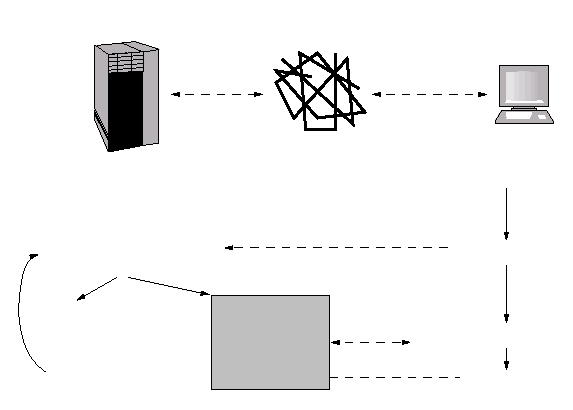
\includegraphics{img/tex/tcp_par}%
\end{picture}%
\setlength{\unitlength}{4144sp}%
%
\begingroup\makeatletter\ifx\SetFigFont\undefined%
\gdef\SetFigFont#1#2#3#4#5{%
  \reset@font\fontsize{#1}{#2pt}%
  \fontfamily{#3}\fontseries{#4}\fontshape{#5}%
  \selectfont}%
\fi\endgroup%
\begin{picture}(4097,2847)(52,-2098)
\put(721,659){\makebox(0,0)[lb]{\smash{\SetFigFont{10}{12.0}{\sfdefault}{\mddefault}{\updefault}{\color[rgb]{0,0,0}server}%
}}}
\put(3736,569){\makebox(0,0)[lb]{\smash{\SetFigFont{10}{12.0}{\sfdefault}{\mddefault}{\updefault}{\color[rgb]{0,0,0}klient}%
}}}
\put(2206,569){\makebox(0,0)[lb]{\smash{\SetFigFont{10}{12.0}{\sfdefault}{\mddefault}{\updefault}{\color[rgb]{0,0,0}s��}%
}}}
\put(406,-511){\makebox(0,0)[lb]{\smash{\SetFigFont{10}{12.0}{\ttdefault}{\mddefault}{\updefault}{\color[rgb]{0,0,0}fd = socket()}%
}}}
\put(631,-691){\makebox(0,0)[lb]{\smash{\SetFigFont{10}{12.0}{\ttdefault}{\mddefault}{\updefault}{\color[rgb]{0,0,0}bind(fd)}%
}}}
\put(541,-871){\makebox(0,0)[lb]{\smash{\SetFigFont{10}{12.0}{\ttdefault}{\mddefault}{\updefault}{\color[rgb]{0,0,0}listen(fd)}%
}}}
\put(271,-1051){\makebox(0,0)[lb]{\smash{\SetFigFont{10}{12.0}{\ttdefault}{\mddefault}{\updefault}{\color[rgb]{0,0,0}fd2 = accept(fd)}%
}}}
\put(631,-1231){\makebox(0,0)[lb]{\smash{\SetFigFont{10}{12.0}{\ttdefault}{\mddefault}{\updefault}{\color[rgb]{0,0,0}fork()}%
}}}
\put(181,-1501){\makebox(0,0)[lb]{\smash{\SetFigFont{10}{12.0}{\ttdefault}{\mddefault}{\updefault}{\color[rgb]{0,0,0}close(fd2)}%
}}}
\put(181,-1666){\makebox(0,0)[lb]{\smash{\SetFigFont{10}{12.0}{\ttdefault}{\mddefault}{\updefault}{\color[rgb]{0,0,0}while(waitpid(}%
}}}
\put(181,-1831){\makebox(0,0)[lb]{\smash{\SetFigFont{10}{12.0}{\ttdefault}{\mddefault}{\updefault}{\color[rgb]{0,0,0}\ \ -1, stat,}%
}}}
\put(181,-1996){\makebox(0,0)[lb]{\smash{\SetFigFont{10}{12.0}{\ttdefault}{\mddefault}{\updefault}{\color[rgb]{0,0,0}\ \ WNOHANG)>0) ;}%
}}}
\put(3331,-511){\makebox(0,0)[lb]{\smash{\SetFigFont{10}{12.0}{\ttdefault}{\mddefault}{\updefault}{\color[rgb]{0,0,0}fd = socket()}%
}}}
\put(3511,-2041){\makebox(0,0)[lb]{\smash{\SetFigFont{10}{12.0}{\ttdefault}{\mddefault}{\updefault}{\color[rgb]{0,0,0}close(fd)}%
}}}
\put(3421,-1051){\makebox(0,0)[lb]{\smash{\SetFigFont{10}{12.0}{\ttdefault}{\mddefault}{\updefault}{\color[rgb]{0,0,0}connect(fd)}%
}}}
\put(1883,-1501){\makebox(0,0)[lb]{\smash{\SetFigFont{10}{12.0}{\sfdefault}{\mddefault}{\updefault}{\color[rgb]{0,0,0}syn}%
}}}
\put(1598,-1681){\makebox(0,0)[lb]{\smash{\SetFigFont{10}{12.0}{\ttdefault}{\mddefault}{\updefault}{\color[rgb]{0,0,0}read(fd2)}%
}}}
\put(1553,-1861){\makebox(0,0)[lb]{\smash{\SetFigFont{10}{12.0}{\ttdefault}{\mddefault}{\updefault}{\color[rgb]{0,0,0}write(fd2)}%
}}}
\put(3106,-1771){\makebox(0,0)[lb]{\smash{\SetFigFont{10}{12.0}{\ttdefault}{\mddefault}{\updefault}{\color[rgb]{0,0,0}write(fd);read(fd)}%
}}}
\put(1666,-2041){\makebox(0,0)[lb]{\smash{\SetFigFont{10}{12.0}{\ttdefault}{\mddefault}{\updefault}{\color[rgb]{0,0,0}exit(0)}%
}}}
\end{picture}

\end{slide}

\begin{itemize}
\item For each client connection the server accepts, a new process is created to
process it.  After the connection is finished, the child exits.  The parent
process can accept new connections meanwhile.  So, multiple connections may be
served in parallel.
\item After \funnm{fork}()ing but before starting to use the connection, the
child may \funnm{exec}() -- that is how \texttt{inetd} works, see page
\pageref{INETD}.
\item As you already know, by calling \funnm{waitpid}() you are getting rid of
zombies. This only works because the \texttt{WNOHANG} flag is used,
otherwise the parent would be blocked and the next connection would only be
accepted after one of the children exited.
Another way is to set to ignore \texttt{SIGCHLD} in which case you
completely avoid the grave danger of the living dead attack (see page
\pageref{IGNORE_SIG_CHLD}).  You could also catch the signal and call
one of the \funnm{wait}() calls from the handler itself which is fine as the
call is async-signal-safe (see page \pageref{ASYNCSIGNALSAFE}).
\end{itemize}

%%%%%

\begin{slide}
\sltitle{Connection-oriented service, parallel \texttt{accept()}}
\begin{picture}(0,0)%
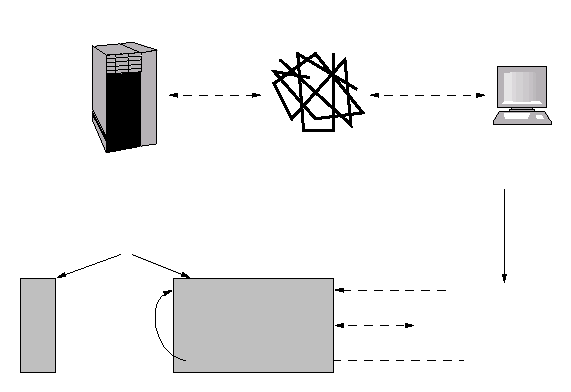
\includegraphics{img/tex/tcp_prefork}%
\end{picture}%
\setlength{\unitlength}{4144sp}%
%
\begingroup\makeatletter\ifx\SetFigFont\undefined%
\gdef\SetFigFont#1#2#3#4#5{%
  \reset@font\fontsize{#1}{#2pt}%
  \fontfamily{#3}\fontseries{#4}\fontshape{#5}%
  \selectfont}%
\fi\endgroup%
\begin{picture}(4070,2712)(79,-1963)
\put(721,659){\makebox(0,0)[lb]{\smash{\SetFigFont{10}{12.0}{\sfdefault}{\mddefault}{\updefault}{\color[rgb]{0,0,0}server}%
}}}
\put(3736,569){\makebox(0,0)[lb]{\smash{\SetFigFont{10}{12.0}{\sfdefault}{\mddefault}{\updefault}{\color[rgb]{0,0,0}klient}%
}}}
\put(1463,-1546){\makebox(0,0)[lb]{\smash{\SetFigFont{10}{12.0}{\ttdefault}{\mddefault}{\updefault}{\color[rgb]{0,0,0}read(fd2)}%
}}}
\put(1418,-1726){\makebox(0,0)[lb]{\smash{\SetFigFont{10}{12.0}{\ttdefault}{\mddefault}{\updefault}{\color[rgb]{0,0,0}write(fd2)}%
}}}
\put(1306,-1366){\makebox(0,0)[lb]{\smash{\SetFigFont{10}{12.0}{\ttdefault}{\mddefault}{\updefault}{\color[rgb]{0,0,0}fd2=accept(fd)}%
}}}
\put(1441,-1906){\makebox(0,0)[lb]{\smash{\SetFigFont{10}{12.0}{\ttdefault}{\mddefault}{\updefault}{\color[rgb]{0,0,0}close(fd2)}%
}}}
\put(676,-1051){\makebox(0,0)[lb]{\smash{\SetFigFont{10}{12.0}{\ttdefault}{\mddefault}{\updefault}{\color[rgb]{0,0,0}fork()}%
}}}
\put(496,-1411){\makebox(0,0)[lb]{\smash{\SetFigFont{20}{24.0}{\ttdefault}{\mddefault}{\updefault}{\color[rgb]{0,0,0}...}%
}}}
\put(2206,569){\makebox(0,0)[lb]{\smash{\SetFigFont{10}{12.0}{\sfdefault}{\mddefault}{\updefault}{\color[rgb]{0,0,0}s��}%
}}}
\put(406,-511){\makebox(0,0)[lb]{\smash{\SetFigFont{10}{12.0}{\ttdefault}{\mddefault}{\updefault}{\color[rgb]{0,0,0}fd = socket()}%
}}}
\put(631,-691){\makebox(0,0)[lb]{\smash{\SetFigFont{10}{12.0}{\ttdefault}{\mddefault}{\updefault}{\color[rgb]{0,0,0}bind(fd)}%
}}}
\put(541,-871){\makebox(0,0)[lb]{\smash{\SetFigFont{10}{12.0}{\ttdefault}{\mddefault}{\updefault}{\color[rgb]{0,0,0}listen(fd)}%
}}}
\put(3331,-511){\makebox(0,0)[lb]{\smash{\SetFigFont{10}{12.0}{\ttdefault}{\mddefault}{\updefault}{\color[rgb]{0,0,0}fd = socket()}%
}}}
\put(3421,-1366){\makebox(0,0)[lb]{\smash{\SetFigFont{10}{12.0}{\ttdefault}{\mddefault}{\updefault}{\color[rgb]{0,0,0}connect(fd)}%
}}}
\put(3106,-1636){\makebox(0,0)[lb]{\smash{\SetFigFont{10}{12.0}{\ttdefault}{\mddefault}{\updefault}{\color[rgb]{0,0,0}write(fd);read(fd)}%
}}}
\put(3511,-1906){\makebox(0,0)[lb]{\smash{\SetFigFont{10}{12.0}{\ttdefault}{\mddefault}{\updefault}{\color[rgb]{0,0,0}close(fd)}%
}}}
\end{picture}

\end{slide}

\begin{itemize}
\item After calling \funnm{bind}() and \funnm{listen}(), the parent creates
several children who sequentially serve connection requests.  Kernel,
from the user point of view in non-deterministic fashion, distributes the
connection requests between child processes waiting in \funnm{accept}().
The parent itself does not serve any connection but possibly \funnm{wait}()s and
creates new processes as needed.
\item The parent should monitor the number of existing children serving
connections and spawn new processes as necessary.
It is a good idea for child processes to voluntarily exit after serving a
certain number of connections to avoid issues like memory leaks to affect the
host as a whole. Apache web server can be configured to work like this.
\item All server side ways of serving the connections work with the same client.
The way a client works does not depend on which approach the server chooses.
\end{itemize}

\begin{slide}
\sltitle{Datagram services (UDP)}
\begin{picture}(0,0)%
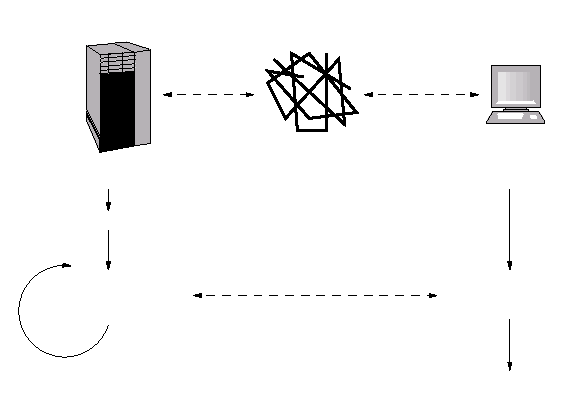
\includegraphics{img/tex/udp}%
\end{picture}%
\setlength{\unitlength}{4144sp}%
%
\begingroup\makeatletter\ifx\SetFigFont\undefined%
\gdef\SetFigFont#1#2#3#4#5{%
  \reset@font\fontsize{#1}{#2pt}%
  \fontfamily{#3}\fontseries{#4}\fontshape{#5}%
  \selectfont}%
\fi\endgroup%
\begin{picture}(4030,2790)(119,-2041)
\put(721,659){\makebox(0,0)[lb]{\smash{\SetFigFont{10}{12.0}{\sfdefault}{\mddefault}{\updefault}{\color[rgb]{0,0,0}server}%
}}}
\put(3736,569){\makebox(0,0)[lb]{\smash{\SetFigFont{10}{12.0}{\sfdefault}{\mddefault}{\updefault}{\color[rgb]{0,0,0}klient}%
}}}
\put(2206,569){\makebox(0,0)[lb]{\smash{\SetFigFont{10}{12.0}{\sfdefault}{\mddefault}{\updefault}{\color[rgb]{0,0,0}s��}%
}}}
\put(338,-511){\makebox(0,0)[lb]{\smash{\SetFigFont{10}{12.0}{\ttdefault}{\mddefault}{\updefault}{\color[rgb]{0,0,0}fd = socket()}%
}}}
\put(563,-817){\makebox(0,0)[lb]{\smash{\SetFigFont{10}{12.0}{\ttdefault}{\mddefault}{\updefault}{\color[rgb]{0,0,0}bind(fd)}%
}}}
\put(473,-1501){\makebox(0,0)[lb]{\smash{\SetFigFont{10}{12.0}{\ttdefault}{\mddefault}{\updefault}{\color[rgb]{0,0,0}sendto(fd)}%
}}}
\put(383,-1321){\makebox(0,0)[lb]{\smash{\SetFigFont{10}{12.0}{\ttdefault}{\mddefault}{\updefault}{\color[rgb]{0,0,0}recvfrom(fd)}%
}}}
\put(3398,-511){\makebox(0,0)[lb]{\smash{\SetFigFont{10}{12.0}{\ttdefault}{\mddefault}{\updefault}{\color[rgb]{0,0,0}fd = socket()}%
}}}
\put(3578,-2041){\makebox(0,0)[lb]{\smash{\SetFigFont{10}{12.0}{\ttdefault}{\mddefault}{\updefault}{\color[rgb]{0,0,0}close(fd)}%
}}}
\put(3533,-1321){\makebox(0,0)[lb]{\smash{\SetFigFont{10}{12.0}{\ttdefault}{\mddefault}{\updefault}{\color[rgb]{0,0,0}sendto(fd)}%
}}}
\put(3443,-1501){\makebox(0,0)[lb]{\smash{\SetFigFont{10}{12.0}{\ttdefault}{\mddefault}{\updefault}{\color[rgb]{0,0,0}recvfrom(fd)}%
}}}
\end{picture}

\end{slide}

\begin{itemize}
\item Note that there is no \funnm{listen} call.
\item Both the client and server use the same functions, the client is one that
sends the first datagram.
\item As in TCP, a client does not need \funnm{bind}() unless it requires a
specific local address to bind to.  The server gets the client address from the
received datagram.
\item In contrast to connection-oriented service, the connection-less one has
less overhead and one can use the same socket to communicate with multiple
remote processes.
\item You can use \funnm{connect}() for UDP as well, see page
\pageref{CONNECT_FOR_UDP} for more information.
\end{itemize}

%%%%%

ifdef([[[NOSPELLCHECK]]], [[[
\pdfbookmark[1]{recvfrom}{recvfrom}
]]])

\begin{slide}
\sltitle{Receiving message: \texttt{recvfrom()}}
\setlength{\baselineskip}{0.8\baselineskip}
ifdef([[[NOSPELLCHECK]]], [[[
\funml{ssize\_t \funnm{recvfrom}(\=int \emph{sock}, void *\emph{buf},
size\_t \emph{l{}en}, \\\>int \emph{flg}, struct sockaddr *\emph{address},
\\\>socklen\_t *\emph{address\_len});}
]]])
\begin{itemize}
\item receives a message from \emph{\texttt{sock}}, stores it to
\emph{\texttt{buf}}
of size \emph{\texttt{l{}en}}, puts the sender's address to \emph{address},
and address length to \emph{\texttt{address\_len}}.  Returns message length.
If the message does not fit \emph{l{}en}, extra data is discarded
(\texttt{SOCK\_STREAM} does not divide data, nothing is discarded).
\item flags \emph{\texttt{flg}} can be:
    \begin{itemize}
    \item \texttt{MSG\_PEEK} \dots{} message it considered not read, next
    \texttt{recvfrom} will return it again
    \item \texttt{MSG\_OOB} \dots{} reads urgent (out-of-band)
    data 
    \item \texttt{MSG\_WAITALL} \dots{} waits for the buffer to fill up
    i.e. \emph{l{}en} bytes
    \end{itemize}
\end{itemize}
\end{slide}

\begin{itemize}
\item Mainly for \texttt{SOCK\_DGRAM} sockets. Waits for the whole message,
does not return datagram portion. Again, it is possible to set the socket
as non-blocking.
\item There does not seem to be a portable way how to get the size of the
UDP datagram before reading it out from kernel buffer. On Linux the
\texttt{MSG\_TRUNC|MSG\_PEEK} flags can be used for \texttt{recvfrom} to get the
size. On other systems the generic \texttt{recvmsg} syscall can be used to at
least provide awareness of the truncation (\texttt{MSG\_TRUNC} flag in the
\texttt{msghdr} structure).
Depending on the application, using large buffer (based on lower network layer
constraints) might be the answer (at the cost of wasting memory).
\item \texttt{address\_len} \emsl{must} be initialized with buffer size if
the address is not \texttt{NULL}. \texttt{NULL} address is used to express that
the caller is not interested in remote's address -- however that is usually
not the case when working with datagrams.
\item Instead of using \texttt{recvfrom} it is possible to use
\texttt{recvmsg} which is more generic.
\item If \texttt{connect} was used then \texttt{recv} can be used instead of
\texttt{recvfrom}.
\item After successful return from \texttt{recvfrom} it is possible to reuse
\texttt{address} and \texttt{address\_len} unchanged for a \texttt{sendto} call.
\item Like \texttt{sendto}, \texttt{recvfrom} is possible to use for connected
service. That said, getting remote's address is better via
\texttt{getpeername}, see page \pageref{GETPEERNAME}.
\item Example: \label{UDP_SERVER_C} \example{udp/udp-server.c}
\end{itemize}

%%%%%

ifdef([[[NOSPELLCHECK]]], [[[
\pdfbookmark[1]{sendto}{sendto}
]]])

\begin{slide}
\sltitle{Sending message: \texttt{sendto()}}
ifdef([[[NOSPELLCHECK]]], [[[
\funml{ssize\_t \funnm{sendto}(\=int \emph{socket}, void *\emph{msg},
size\_t \emph{l{}en},\\\>int \emph{flags}, struct sockaddr *\emph{addr},
\\\>socklen\_t \emph{addr\_len});}
]]])
\begin{itemize}
\item sends a message \emph{\texttt{msg}} via \emph{socket} of \emph{l{}en}
bytes to address \emph{\texttt{addr}} (of \emph{\texttt{addr\_len}} length). 
\item \emph{flags} can carry:
    \begin{itemize}
    \item \texttt{MSG\_EOB} \dots{} finish a record (if supported by the
    protocol)
    \item \texttt{MSG\_OOB} \dots{} send urgent (out-of-band) data
    \end{itemize}
\end{itemize}
\end{slide}

\begin{itemize}
\item Used mainly for \texttt{SOCK\_DGRAM} sockets, because in such situation
we only have socket representing our side of the connection; see the note
for \texttt{accept}. The remote address has to be specified which cannot be
done with \texttt{write}. Moreover, for \emsl{datagram} service the data sent
is considered as whole, i.e. either it is accepted completely or the call
will block -- partial write does not exist. Like with file descriptors, it is
possible to set the socket as non-blocking, see page \pageref{FCNTL}.
\item Instead of using \texttt{sendto} more generic function \texttt{sendmsg}
can be used.
\item If \texttt{connect} was used then \texttt{send} can be used instead of
\texttt{sendto}.
\item Successful return from either \emsl{does not mean successful delivery of
the message to the remote side}, but only insertion of the data to local buffer
which is yet to be sent out.
\item It is possible to use \texttt{sendto} for stream service, however the
address will be ignored. The only reason not to use \texttt{write} would be to
use flags. In this case it is simpler to use \texttt{send}.
\item Example:\label{UDP_CLIENT_C} \example{udp/udp-client.c}.
\end{itemize}

%%%%%

\pdfbookmark[1]{close}{close}

\begin{slide}
\sltitle{Closing socket: \texttt{close()}}
\setlength{\baselineskip}{0.8\baselineskip}
\texttt{int \funnm{close}(int \emph{sock});}
\begin{itemize}
\item close descriptor \emph{sock}, after the last descriptor is closed, close
the socket in kernel
\item for the \texttt{SOCK\_STREAM} socket,
\texttt{SO\_LINGER} flag is important (default is \texttt{.l\_onoff~==~0}, use
\funnm{setsockopt}() with \texttt{struct linger} to change that).
    \begin{itemize}
    \item \texttt{.l\_onoff~==~0} \dots{} \funnm{close}() returns but system
    tries to transfer rest of the data
    \item \texttt{.l\_onoff~==~1~\&\&~.l\_linger~!=~0} \dots{} system tries to
    transfer data until timeout \texttt{l\_linger} expires (in seconds), if it
    fails, return error, otherwise return OK after transferring data.
    \item \texttt{.l\_onoff~==~1~\&\&~.l\_linger~==~0} \dots{} reset the
    connection
    \end{itemize}
\end{itemize}
\end{slide}

\label{CLOSESOCKET}

\begin{itemize}
\item Once closed, TCP socket can remain in transitory state which is defined in
TCP protocol for connection closing. Before the socket is completely destroyed,
it is not possible to use another socket with the same port, unless this
behavior was overridden with the \texttt{SO\_REUSEADDR} flag using the
\texttt{setsockopt} function, see page \pageref{SETSOCKOPT}.
\item Connection reset is abnormal connection termination. In case of TCP
a packet with \texttt{RST} flag is used for such termination. The remote side
will detect this as end of file when reading, the reset will lead to the
\texttt{ECONNRESET} error. Example: \example{tcp/linger.c}.
\end{itemize}

%%%%%

\pdfbookmark[1]{shutdown}{shutdown}

\begin{slide}
\sltitle{Shut down part of a connection: \texttt{shutdown()}}
\texttt{int \funnm{shutdown}(int \emph{socket}, int \emph{how});}
\begin{itemize}
\item shuts down a socket but does not close the descriptor, \emph{how} can be: 
    \begin{itemize}
    \item \texttt{SHUT\_RD} \dots{} shut it down for reading
    \item \texttt{SHUT\_WR} \dots{} for writing
    \item \texttt{SHUT\_RDWR} \dots{} for both
    \end{itemize}
\end{itemize}
\end{slide}

\begin{itemize}
\item After using \texttt{shutdown} it is still necessary to close the
descriptor using \texttt{close}.
\item Normal TCP connection termination each side will signal that no subsequent
writes will follow. This is valid for either \texttt{close} or
\texttt{shutdown(fd, SHUT\_RDWR)}. When using
\texttt{shutdown(fd, SHUT\_WR)} it is still possible to read from the socket.
The remote side will get \texttt{EOF} while reading however it can still write.
\end{itemize}

%%%%%

ifdef([[[NOSPELLCHECK]]], [[[
\pdfbookmark[1]{inet\_pton, inet\_ntop}{ipaddrfncs}
]]])

\begin{slide}
\sltitle{Working with IPv4 and IPv6 addresses}
\begin{itemize}
\item binary representation of IP address is hard to read
\item string representation of IP address cannot be used when working with
\texttt{sockaddr} structures
\end{itemize}
ifdef([[[NOSPELLCHECK]]], [[[
\texttt{int \funnm{inet\_pton}(int \emph{af}, const char *\emph{src},
void *\emph{dst});}
]]])
\begin{itemize}
\item converts string to binary representation, i.e. something usable for
\texttt{in\_addr} or \texttt{in6\_addr} members of \texttt{sockaddr} structures
\item returns 1 (OK), 0 (wrong address) or -1 (and sets \texttt{errno})
\end{itemize}
ifdef([[[NOSPELLCHECK]]], [[[
\funml{cont char *\funnm{inet\_ntop}(\=int \emph{af}, const void *\emph{src},
\\\>char *\emph{dst}, size\_t \emph{size});}
]]])
\begin{itemize}
\item counterpart to \texttt{inet\_pton}; returns \emph{\texttt{dst}} or
\texttt{NULL} (and sets \texttt{errno})
\end{itemize}
\begin{itemize}
\item for both functions \texttt{af} is either \texttt{AF\_INET} or
\texttt{AF\_INET6}
\end{itemize}
\end{slide}

\label{IPv4_IPv6_ADDRESSES}

\begin{itemize}
\item The functions are declared in \texttt{arpa/inet.h}.
\item \texttt{inet\_pton} returns 1 if the conversion successfully happened,
0 if given string is not an address or -1 if \emph{\texttt{af}} is not supported
(\texttt{EAFNOSUPPORT}). \texttt{inet\_ntop} returns \texttt{dst} if everything
is OK otherwise returns \texttt{NULL} with \texttt{errno} set.
\item Addresses and ports in binary form are stored as big endian.
\item \texttt{dst} has to be sufficiently sized because there is no parameter
specifying the size. This is not a problem since according to the value of
\texttt{af} appropriate address structure or character array can be passed in.
For maximal lengths of strings for addresses, 2 macros can be used --
\texttt{INET\_ADDRSTR\-LEN} (16) or \texttt{INET6\_ADDRSTRLEN} (48). 
These values contain space for terminating \texttt{\bs{}0}.
\item \texttt{size} is string size of \texttt{dst}. If not sufficient, the call
will fail and \texttt{ENOSPC} will be set.
\item \texttt{n} stands for \texttt{network}, \texttt{p} stands for
\texttt{presentable}
\item In the past \texttt{inet\_aton} and \texttt{inet\_ntoa} (\texttt{a} as
\texttt{ascii}) were used for IPv4 addresses. Thanks for the functions above
these are now legacy. All these calls are usually documented in the
\texttt{inet} man page.
\item \label{ADDRESSES} Do realize that using these functions it is only
possible to convert one address family once, either IPv4 or IPv6.
When the output can be either, try one and if that fails, fallback to another.
Example: \example{resolving/addresses.c}.
\end{itemize}

%%%%%

ifdef([[[NOSPELLCHECK]]], [[[
\pdfbookmark[1]{setsockopt, getsockopt, getsockname, getpeername}{socketfncs}
]]])

\begin{slide}
\sltitle{More socket functions}
ifdef([[[NOSPELLCHECK]]], [[[
\funml{int \funnm{setsockopt}(\=int \emph{socket}, int \emph{level},
int \emph{opt\_name}, \\\>const void *\emph{opt\_value},
socklen\_t \emph{option\_len});}
]]])
\begin{itemize}
\item sets socket parameters
\end{itemize}
ifdef([[[NOSPELLCHECK]]], [[[
\funml{int \funnm{getsockopt}(\=int \emph{socket}, int \emph{level},
int \emph{opt\_name},\\\>void *\emph{opt\_value},
socklen\_t *\emph{option\_len});}
]]])
\begin{itemize}
\item reads socket parameters
\end{itemize}
ifdef([[[NOSPELLCHECK]]], [[[
\funml{int \funnm{getsockname}(\=int \emph{socket},
struct sockaddr *\emph{address}, \\\>socklen\_t *\emph{address\_len});}
]]])
\begin{itemize}
\item get local socket address
\end{itemize}
ifdef([[[NOSPELLCHECK]]], [[[
\funml{int \funnm{getpeername}(\=int \emph{socket},
struct sockaddr *\emph{address}, \\\>socklen\_t *\emph{address\_len});}
]]])
\begin{itemize}
\item get address of the remote end
\end{itemize}
\end{slide}

\label{SETSOCKOPT}
\label{GETPEERNAME}
\label{GETSOCKOPT}

\begin{itemize}
\item The \texttt{level} value for \texttt{getsockopt} and \texttt{setsockopt}
is usually \verb#SOL_SOCKET#. For \texttt{get\-sock\-opt},
the \texttt{option\_len} value \emsl{must} be initialized to
the size of \texttt{opt\_value}.
\item \texttt{getsockname} is used when not using \texttt{bind} syscall
to determine what is the (local !) address assigned to the socket by the kernel.
\item ifdef([[[NOSPELLCHECK]]],
[[[\verb#getsockopt(sock, SOL_SOCKET, SO_ERROR, &val, &len)#]]]) returns
(and erases) error indication for given socket. This is mainly useful to
get result of non-blocking \texttt{connect}, see page \pageref{CONNECT}.
\item When using ifdef([[[NOSPELLCHECK]]], [[[\verb#SO_REUSEADDR#]]]) it is
possible to immediately create new server (i.e. to successfully call
\texttt{socket},
\texttt{bind}, \texttt{listen} and \texttt{accept}) listening on address and
port previously used even though there are still TCP connections in their final
stage from the previous instance of the server:

\begin{verbatim}
int opt = 1;
setsockopt(fd, SOL_SOCKET, SO_REUSEADDR, &opt, sizeof(opt));
\end{verbatim}

\item See \verb#SO_REUSEADDR# being used in example \example{tcp/reuseaddr.c}.
For the demonstration it is necessary to establish at least once connection,
otherwise there is nothing to wait for and repeated \texttt{bind} will succeed
anyway.
\end{itemize}

%%%%%

ifdef([[[NOSPELLCHECK]]], [[[
\pdfbookmark[1]{htonl, ntohl, htons, ntohs}{byteorderfncs}
]]])

\begin{slide}
\sltitle{Byte order}
\begin{itemize}
\item network services can use byte ordering that differs from the native
one on the system. Conversion functions (macros):
    \begin{itemize}
    ifdef([[[NOSPELLCHECK]]], [[[
    \item\texttt{uint32\_t \funnm{htonl}(uint32\_t \emph{hostlong});}\\
    ]]]) host $\rightarrow$ network, 32 bits
    ifdef([[[NOSPELLCHECK]]], [[[
    \item\texttt{uint16\_t \funnm{htons}(uint16\_t \emph{hostshort});}\\
    ]]]) host $\rightarrow$ network, 16 bits
    ifdef([[[NOSPELLCHECK]]], [[[
    \item \texttt{uint32\_t \funnm{ntohl}(uint32\_t \emph{netlong});}\\
    ]]]) network $\rightarrow$ host, 32 bits
    ifdef([[[NOSPELLCHECK]]], [[[
    \item \texttt{uint16\_t \funnm{ntohs}(uint16\_t \emph{netshort});}\\
    ]]]) network $\rightarrow$ host, 16 bits 
    \end{itemize}
\item network byte order is big-endian, i.e. most significant byte first.
Both network addresses and port numbers are multibyte values.
\end{itemize}
\end{slide}

\label{HTON}

\begin{itemize}
\item If the local system uses the network byte order natively, the functions
become no-ops.
\item Simple and sufficient test is to run your program in 2 instances 
against each other (if possible) on two systems with different endianess.
\end{itemize}

%%%%%

ifdef([[[NOSPELLCHECK]]], [[[
\pdfbookmark[1]{getprotobyname, getservbyname}{protonumfncs}
]]])

\begin{slide}
\sltitle{Protocol and port numbers}
ifdef([[[NOSPELLCHECK]]], [[[
\texttt{struct protoent *\funnm{getprotobyname}(const char *\emph{name});}
]]])
\begin{itemize}
\item returns protocol number in \texttt{p\_proto} with \emph{name}
(e.g. for \texttt{"tcp"} returns 6).
\item protocol numbers are stored in the \texttt{/etc/protocols} file.
\end{itemize}
ifdef([[[NOSPELLCHECK]]], [[[
\funml{struct servent *\funnm{getservbyname}(\=const char *\emph{name},
\\\>const char *\emph{proto});}
]]])
\begin{itemize}
\item for service name \texttt{name} and protocol name \texttt{proto}
returns port number in \texttt{s\_port}.
\item port numbers are stored in the \texttt{/etc/services} file.
\end{itemize}

The functions return \texttt{NULL}, if matching entry cannot be find in the
database.
\end{slide}

\begin{itemize}
\item The result of \funnm{getprotobyname} is handy for calling \texttt{socket},
the result of \funnm{getservbyname} is for \texttt{bind}.
\item Next to \texttt{getservbyname} there is also \texttt{getservbyport}
that finds service entry according to port number (in network byte order !)
and function \texttt{getservent} and others. for entry traversal.
\item All these functions search only "official" lists of services and
protocols, which are located in the relevant naming databases (see slide on
page \pageref{name_service_switch}). Note that the slide mentions the files for
simplification.
\item These files define the mapping for names and numbers for standard
protocols and services.
\item Keep in mind that protocol is the upper layer protocol as specified in
the IP packet header, (e.g. TCP, UDP, OSPF, GRE etc., see pages 11 and 14 in
RFC~791), not HTTP, SSH, telnet or FTP -- these are \emph{services}, represented
by port numbers.
\item \label{GETBYNAME} example: \example{resolving/getbyname.c}
\end{itemize}

%%%%%

ifdef([[[NOSPELLCHECK]]], [[[
\pdfbookmark[1]{getaddrinfo}{getaddrinfo}
]]])

\label{GETADDRINF}

\begin{slide}
\sltitle{Convert hostname to addresses: \texttt{getaddrinfo()}}

\begin{itemize}
\item generates \texttt{sockaddr} structures from given parameters
\item works with both IP addresses and ports
\item can influence the behavior with \emph{hints}

ifdef([[[NOSPELLCHECK]]], [[[
\funml{int \funnm{getaddrinfo}(\=const char *\emph{nodename},
\\\>const char *\emph{servicename},
\\\>const struct addrinfo *\emph{hint},
\\\>struct addrinfo **\emph{res});}
]]])
\item \texttt{addrinfo} structure members:
\texttt{ai\_flags} (for hints), \texttt{ai\_family} (address family),
\texttt{ai\_socktype}, \texttt{ai\_protocol}, \texttt{ai\_addrlen},
\texttt{struct sockaddr *ai\_addr} (resulting addresses),
\texttt{char *ai\_canonname},
\texttt{struct addrinfo *ai\_next} (next item in the list)
\end{itemize}
\end{slide}

\begin{itemize}
\item When evaluating queries for addresses and names, the naming services
are consulted according to the specification in the \texttt{/etc/nsswitch.conf}
file.
\item The structure \texttt{addrinfo} is defined in \texttt{netdb.h}.
\item \texttt{getaddrinfo} is able to convert a string containing either a
hostname or an IP address. Similarly for ports.  So, whether you use a hostname
or an IP address as an command line argument, you can use the same code to
process that.
\item The \texttt{getaddrinfo} function returns the results in the \emph{res}
parameter. The result is a list of \texttt{sockaddr} structures corresponding to
given input.
\item There is a difference whether the address structures are to be used for a
server or client; e.g. for a server it is sufficient to specify \emph{nodename}
as \texttt{NULL} (meaning any address).  Similarly for the member
\texttt{ai\_flags} of the \texttt{addrinfo} structure used for the \emph{hint}
parameter -- for a server, use \texttt{AI\_PASSIVE} to indicate the returned
address structures will be used in \funnm{bind}.
\item After the results are no longer needed, it is prudent to call
\texttt{freeaddrinfo}, that will free the memory allocated by
\texttt{getaddrinfo}.
\item \label{GETADDRINFO} example: \example{resolving/getaddrinfo.c}
\item In the past the functions \funnm{gethostbyname} and
\funnm{gethostbyaddr} were used. These only work with IPv4 addresses and are
therefore considered legacy and not recommended to use. The functions
\funnm{getipnodebyname} and \funnm{get\-ip\-no\-de\-by\-addr} can be used
instead (\funnm{getipnode*} are found in many systems, nevertheless they were
removed from GNU \texttt{libc}, so cannot be relied on universally). What is
more, they are not part of UNIX standards.  \funnm{get\-addr\-info} and
\funnm{getnameinfo} are part of the POSIX.1-2001 standard.
\item It is not strictly necessary to convert old IPv4 specific code to the
generic APIs. However when writing new code, always use them even when you think
the program will only use IPv4.
\item IPv6 sockets may be used for both IPv4 and IPv6 communications.  That
means if you try to bind addresses returned by \funnm{getaddrinfo}, \funnm{bind}
should return \texttt{EADDRINUSE} after its first call if you use both IPv4 and
IPv6 addresses.  Binding on an IPv6 address should be sufficient to accept
connections over IPv4 as well.  Details are in RFC~3493.  If you want to
restrict a socket to IPv6 only, use the following code on a socket from the
\texttt{AF\_INET6} family:

\begin{verbatim}
      int on = 1;

      if (setsockopt(s, IPPROTO_IPV6, IPV6_V6ONLY, (char *)&on,
          sizeof(on)) == -1) {
              /* deal with the error here */
      }
\end{verbatim}

\end{itemize}

%%%%%%

ifdef([[[NOSPELLCHECK]]], [[[
\pdfbookmark[1]{getnameinfo}{getnameinfo}
]]])

\begin{slide}
\sltitle{Convert address to hostname: \texttt{getnameinfo()}}

\begin{itemize}
\item counterpart to \texttt{getaddrinfo}
\item gets \texttt{sockaddr} structures, therefore works with both
IPv4 and IPv6 addresses, as opposed to the \texttt{gethostbyaddr} function.
\end{itemize}
ifdef([[[NOSPELLCHECK]]], [[[
\funml{int \funnm{getnameinfo}(\=const struct sockaddr *\emph{sa},
\\\>socklen\_t *\emph{sa\_len},
\\\>char *\emph{nodename},
\\\>socketlen\_t *\emph{nodelen},
\\\>char *\emph{servicename},
\\\>socketlen\_t *\emph{servicelen},
\\\>unsigned \emph{flags});}
]]])
\end{slide}

\begin{itemize}
\item \texttt{getnameinfo} converts IP address and port number from the
\texttt{sockaddr} structure to strings according to configured name services
(\texttt{/etc/nsswitch.conf}) and the \texttt{flags} value.
It performs the actions that would have to be otherwise done by
\texttt{gethostbyaddr} and \texttt{getservbyport}.
\item Either \texttt{nodename} or \texttt{portname} can be \texttt{NULL} --
that means the caller is not interested in its resolution.
\item Unlike the above mentioned legacy functions \texttt{getnameinfo} is
reentrant and is therefore safe to use with threads.
\item The man page for \texttt{getnameinfo} contains the list of usable
\texttt{NI\_} flags for the \texttt{\emph{flags}} parameter.
\item \label{GETNAMEINFO} example: \example{resolving/getnameinfo.c}


\end{itemize}

%%%%%

\pdfbookmark[1]{TCP server}{tcpservercode}
\label{TCPSRVEXAMPLE}

\begin{slide}
\sltitle{Example: TCP server}
\setlength{\baselineskip}{0.9\baselineskip}
\begin{alltt}
struct sockaddr\_storage ca; int nclients = 10, fd, nfd;
struct addrinfo *r, *rorig, hi;
memset(&hi, 0, sizeof (hi)); hi.ai\_family = AF\_UNSPEC;
hi.ai\_socktype = SOCK\_STREAM; hi.ai\_flags = AI\_PASSIVE;
\emprg{getaddrinfo}(NULL, portstr, &hi, &rorig);
for (r = rorig; r != NULL; r = r->ai\_next) \{
    fd = \emprg{socket}(r->ai\_family, r->ai\_socktype,
        r->ai\_protocol);
    if (!\emprg{bind}(fd, r->ai\_addr, r->ai\_addrlen)) break;
\}
\emprg{freeaddrinfo}(rorig); \emprg{listen}(fd, nclients);
for (;;) \{ sz = sizeof(ca);
    nfd = \emprg{accept}(fd, (struct sockaddr *)&ca, &sz);
    /* communication with the client */
    close(newsock);
\}
\end{alltt}
\end{slide}

\begin{itemize}
\item This is generic skeleton of TCP server. The \texttt{portstr} parameter
is the only input value of the program. First successful \texttt{bind} will
finish traversal of the IP address list.
\item Program written in such a way will work on system with IPv6 and IPv4
addresses, i.e. it will be able to accept connections for both address families
on the same socket. The remote address of IPv4 clients will be represented as
\emph{IPv4-mapped IPv6 address}, (i.e. it contains embedded IPv4 address, e.g.
e.g. \texttt{::FFFF:78.128.192.1}).
\item Note that it is mostly not necessary to cast to the \texttt{sockaddr}
structure. The only exception is the \texttt{accept} call.
For the \texttt{accept} call the \texttt{sockaddr\_storage} is used which is
generic "container" able to store members of both \texttt{sockaddr\_in} and
\texttt{sockaddr\_in6} structures.
\item \texttt{socket} and \texttt{bind} are called for all returned
\texttt{sockaddr} structures until \texttt{bind} succeeds for one of them
or the list is not finished.
\item The code on the slide does not check all return values and does not
free all the allocated entities, e.g. socket closing in case of \texttt{bind}
error. Also, it does not deal with the situation when the list of addresses
is traversed without successful \texttt{bind} (this can be detected
with \texttt{r} NULL check after the end of the first cycle).
\end{itemize}

%%%%%

\pdfbookmark[1]{TCP client}{tcpclientcode}
\label{TCPCLNTEXAMPLE}

\begin{slide}
\sltitle{Example: TCP client}
\begin{alltt}
int fd; struct addrinfo *r, *rorig, hi;
memset(&hi, 0, sizeof (hi)); hi.ai\_family = AF\_UNSPEC;
hi.ai\_socktype = SOCK\_STREAM;
\emprg{getaddrinfo}(hoststr, portstr, &hi, &r);
for (rorig = r; r != NULL; r = r->ai\_next) \{
    fd = \emprg{socket}(r->ai\_family, r->ai\_socktype,
        r->ai\_protocol);
    if (\emprg{connect}(fd, (struct sockaddr *)r->ai\_addr,
        r->ai\_addrlen) == 0)
            break;
\}
\emprg{freeaddrinfo}(resorig);
/* communication with server */
close(fd);
\end{alltt}
\end{slide}

\begin{itemize}
\item This is generic TCP client skeleton. The \texttt{hoststr} and
\texttt{portstr} arguments are the only input data of the program.
First successful \texttt{connect} will terminate the address traversal
for given host.
\item In the example we let the kernel will choose local port.
(there is no \texttt{bind} before the \texttt{connect}).
\item \texttt{connect} is called sequentially on all returned
\texttt{sockaddr} structures (embedded in the \texttt{addrinfo} structures)
for given host until a connection succeeds or the list is exhausted.
\item Same lack of error checking and freeing or resources as for the TCP
server example, i.e. in situation when the list is exhausted without successful
\texttt{connect}. Also the socket is not closed when \texttt{connect} is not
successful.
\end{itemize}

%%%%%

\pdfbookmark[1]{select}{select}

\begin{slide}
\sltitle{Waiting for data: \texttt{select()}}
\setlength{\baselineskip}{0.9\baselineskip}
ifdef([[[NOSPELLCHECK]]], [[[
\funml{int \funnm{select}(\=int \emph{nfds}, fd\_set *\emph{readfds},
\\\>fd\_set *\emph{writefds}, fd\_set *\emph{errorfds},
\\\>struct timeval *\emph{timeout});}
]]])
\begin{itemize}
\item determines which out of given file descriptors are ready for reading,
writing or which experienced exceptional state. If no such descriptor is
found, waits till \texttt{timeout} expires.
(\texttt{NULL} \dots means arbitrary long wait). The \texttt{nfds} parameter
sets the range of file descriptor values
ifdef([[[NOSPELLCHECK]]], [[[(\texttt{0,~...,~\emsl{nfds-1}}).]]])
\item functions for setting file descriptor masks:
    \begin{itemize}
    ifdef([[[NOSPELLCHECK]]], [[[
    \item \texttt{void \funnm{FD\_ZERO}(fd\_set *\emph{fdset})} \dots{}
    ]]]) initialization
    ifdef([[[NOSPELLCHECK]]], [[[
    \item \texttt{void \funnm{FD\_SET}(int \emph{fd}, fd\_set *\emph{fdset})}
    ]]]) \dots set
    ifdef([[[NOSPELLCHECK]]], [[[
    \item \texttt{void \funnm{FD\_CLR}(int \emph{fd}, fd\_set *\emph{fdset})}
    ]]]) \dots{} unset
    ifdef([[[NOSPELLCHECK]]], [[[
    \item \texttt{int \funnm{FD\_ISSET}(int \emph{fd}, fd\_set *\emph{fdset})}
    ]]]) \dots{} test
    \end{itemize}
\end{itemize}
\end{slide}

\label{SELECT}

\begin{itemize}
\item \emsl{Motivation:} to read data from multiple file descriptors, it is
possible to open respective files with the \texttt{O\_NONBLOCK} flag
(or set the flag after \texttt{open} with \texttt{fncnl} -- with the second
parameter being \texttt{O\_SETFL}, not \texttt{O\_SETFD}, see page
\pageref{FCNTL}).  Repetitious \texttt{read} (which is non-blocking after we set
the descriptor as non-blocking, see page \pageref{OPEN}) is then called on all
descriptors.  Sleeping in every loop is needed in order not to hammer the kernel
with syscalls.  For every invocation, you either read some data right away or get
\texttt{-1} with \texttt{errno} set to \texttt{EAGAIN} if no data was ready,
meaning the call would have blocked if it was not for the non-blocking
descriptor.  However, the disadvantages are: active waiting, frequent
user-kernel mode switching, possible delay (up to the wait period between the
iterations of the cycle).  Correct solution of this situation is to use e.g.
\texttt{select} and then call \texttt{read} only for those descriptors marked as
\emph{ready}.
\item \label{BUSY_WAITING_C} Busy waiting example: \example{select/busy-wait.c}.
Notice that newly created socket does not have the \texttt{O\_NONBLOCK} flag,
see page \pageref{ACCEPT}, so it is necessary to set it.
\item A descriptor marked as \emph{ready} means that \texttt{read} or
\texttt{write} on this descriptor with a cleared \texttt{O\_NONBLOCK} flag would
not block, therefore there has to be some data ready or some other condition is
pending (\texttt{read} can e.g. return 0 for end-of-file or \texttt{-1} for
error).
\item The set \texttt{errorfds} is for exceptions depending on descriptor type;
for socket it is the reception of urgent data (the \texttt{URG} flag in TCP
header). It does not mean that there was an error on given descriptor.  The
error is determined by checking \texttt{errno} after given syscall returns
\texttt{-1}.
\item Before calling \texttt{select} the sets contain descriptors of interest,
after the syscall returns the sets contain only those descriptors for which 
specified event happened.  \emsl{It is therefore necessary to refresh the sets
before next call to \texttt{select}.} Typically the sets are implemented as bit
masks however it does not have to be so. The programmer does not have to deal
with that. Traversing the sets is only possible one bit at a time and using
\texttt{FD\_ISSET}.
\item \texttt{select} is handy also for the possibility to write into a pipe or
socket -- waiting for the other side to consume part of the buffer and thus free
space for more incoming data.
\item It is possible to use \texttt{NULL} instead of the descriptor set. Special
case is to use \texttt{NULL} for all the sets in which case the syscall will
block until the timeout expires or a signal is delivered.
\item After returning it is necessary to test each descriptor individually,
there is no call that would create a set of ready descriptors.
\item If networking server handles multiple ports, it is possible to call
\texttt{select} with respective socket descriptors and then \texttt{accept}
for descriptors that \texttt{select} marked as ready, i.e. there is a client
connection waiting (reading readiness).
\item \texttt{connect} on non-blocking socket will return immediately, the
actual connection establishment will be reported by \texttt{select} as readiness
for writing. See page \pageref{CONNECT}.
\item Another possibility to use \texttt{select} is networking server that
handles multiple clients in single process. Using \texttt{select} the client
descriptors are tested and those which are ready are then used for
communication. To allow new clients, the descriptor used for \texttt{accept} is
tested as well.
\item Beware that \texttt{select} \emsl{can} change the \texttt{timeval}
structure; there is a call \texttt{pselect}, that will not change the structure
(besides having other properties).
\item It is possible to use \texttt{FD\_SETSIZE} for the \emsl{\texttt{nfds}}
parameter which is system constant for maximal file descriptor count. This is
not the best solution since this constant is only 1024 on 32-bit systems however
for 64-bit programs it can be significantly bigger (e.g. 65536 on Solaris),
leading to more time spent in the syscall.
\item If the time argument is set to 0 (not NULL), then \texttt{select} can be
used for so called \emph{polling} -- it will check the current state and return
immediately.
\item Example: \label{SELECT_C} \example{select/select.c}
\item \texttt{select} can also be used to determine the state after
\texttt{connect} for non-blocking socket. Use \texttt{getsockopt} with
\texttt{opt\_name} set to \texttt{SO\_ERROR}, (see page \pageref{GETSOCKOPT}) to
see if the connection was successful.
\label{NON_BLOCKING_CONNECT} Example: \example{select/non-blocking-connect.c}.


\end{itemize}

%%%%%

\begin{slide}
\sltitle{Example: \texttt{select()}}
\begin{itemize}
\item The \texttt{fd} descriptor is a socket, converts socket communication
to terminal and ifdef([[[NOSPELLCHECK]]], [[[vice versa]]]).
\end{itemize}
\setlength{\baselineskip}{0.8\baselineskip}
\begin{alltt}
int sz; fd\_set rfdset, efdset; char buf[BUFSZ];
for(;;) \{
    \emprg{FD\_ZERO}(&rfdset); \emprg{FD\_SET}(0, &rfdset);
    \emprg{FD\_SET}(fd, &rfdset); efdset = rfdset;
    \emprg{select}(fd+1, &rfdset, NULL, &efdset, NULL);
    if(\emprg{FD\_ISSET}(0, &efdset))
        /* exception on stdin */ ;
    if(\emprg{FD\_ISSET}(fd, &efdset))
        /* exception on fd */ ;
    if(\emprg{FD\_ISSET}(0, &rfdset)) \{
        sz = read(0, buf, BUFSZ); write(fd, buf, sz); \}
    if(\emprg{FD\_ISSET}(fd, &rfdset)) \{
        sz = read(fd, buf, BUFSZ); write(1,buf,sz); \}
\}
\end{alltt}
\end{slide}

\begin{itemize}
\item Here is typical use of \texttt{select}, when it is necessary to read the
data from two sources. This example assumes that the descriptors
\texttt{0} and \texttt{fd} are set as non-blocking.
\item Better solution would be to use \texttt{select} also for testing writing
readiness. For this two buffers are required -- one for each direction of
communication. Respective read descriptor will be present in the read set for
\texttt{select} when the buffer is empty. The write descriptor will be in the
write set when the buffer is non-empty.
\item \label{WRITE_SELECT_C} \texttt{select} will put the process to sleep
when the data is not read from the remote side if only testing write readiness.
This can be simply simulated by a program that merely connects (TCP handshake)
however does not read anything. Example: \example{select/write-select.c}.
\end{itemize}

%%%%%

ifdef([[[NOSPELLCHECK]]], [[[
\pdfbookmark[1]{poll}{poll}
]]])

\begin{slide}
\sltitle{Waiting for data: \texttt{poll()}}
ifdef([[[NOSPELLCHECK]]], [[[
\texttt{int \funnm{poll}(struct pollfd \emph{fds}[], nfds\_t \emph{nfds},
int \emph{timeout});}
]]])
\begin{itemize}
\item waits for event on one of the descriptors in the \texttt{fds} array
of \texttt{nfds} items for \texttt{timeout} ms (\texttt{0}
\dots{} returns immediately, \texttt{-1} \dots{} waits arbitrarily long).
\item \texttt{pollfd} structure members:
    \begin{itemize}
    \item \texttt{fd} \dots{} descriptor number
    \item \texttt{events} \dots{} events to wait for, OR-combination of
    \texttt{POLLIN} (can read), \texttt{POLLOUT} (can write), etc. 
    \item \texttt{revents} \dots{} events that happened on the descriptor,
    same indications as in \texttt{events}, plus e.g. \texttt{POLLERR}
    (error happened)
    \end{itemize}
\end{itemize}
\end{slide}

\label{POLL}

\begin{itemize}
\item Alternative to \texttt{select}.
\item The \emph{timeout} argument is in milliseconds.
\item There are many more flags, see the man page.
\item Often either \texttt{select} or \texttt{poll} is implemented using the
other one.  On Solaris, for example, \texttt{poll} is a system call, and
\texttt{select} is then a library call implemented as a \texttt{poll} wrapper.
\item \texttt{poll} is necessary to use to test descriptor equal or higher than
\texttt{FD\_SETSIZE}.
\item Unlike \texttt{select} it is not necessary to refresh descriptor sets
after each call or nullify \texttt{revents}. To deselect a file descriptor,
set the \texttt{fd} member of the \texttt{pollfd} structure to -1
(or reshuffle the array which is significantly more complex).
\item Time set to -1 has the same effect as \texttt{NULL} for \texttt{select}.
\item If the number of descriptors is set to 0 (\texttt{fds} should be then
\texttt{NULL}), \texttt{poll} can be simply used to sleep with less than one
second granularity. Example: \label{POLL_SLEEP_C} \example{sleep/poll-sleep.c}
That said, this "trick" does not work on macOS.
\begin{itemize}
\item Another way is to use \texttt{nanosleep}, that is part of POSIX.4
extension and therefore does not have to be always available.
Example: \example{sleep/nanosleep.c}.
\end{itemize}
\item While \texttt{select} and \texttt{poll} are pretty efficient when handling
many connections in parallel, internally they both have $O(n)$ algorithms
inside. The famous "C10k" problem (\url{http://www.kegel.com/c10k.html}),
is about finding a solution on how to efficiently handle tens of thousands of
connections (could be both server and client side - e.g. imagine web crawler) in
parallel. Pretty much all Unix systems offer some sort of event driven library
and/or kernel primitives to achieve that. Also, there are many ways how to
approach the problem, plus some tricks that can be applied on the top.
\end{itemize}

\endinput
